\documentclass[pdf,14pt]{beamer}
\usetheme{default}
\mode<presentation>{}

\usepackage{verbatim}
\usepackage{color}

\begin{document}

\begin{frame}{The Quine}
  \begin{definition}
    A quine is a computer program which takes no input and produces a copy of its own source code as its only output.
  \end{definition}

  \[
    T_u(\left< P \right>) = \left< P \right>
  \]  
\end{frame}

\begin{frame}
  \begin{figure}[ht]
    \begin{center}
      
\includegraphics[width=10cm]{dawg.jpeg}
    \end{center}
  \end{figure}
\end{frame}

\begin{frame}{Quine, Yo}
  \begin{columns}
    \column{0.5\textwidth}
    \begin{figure}[ht]
      \begin{center}
        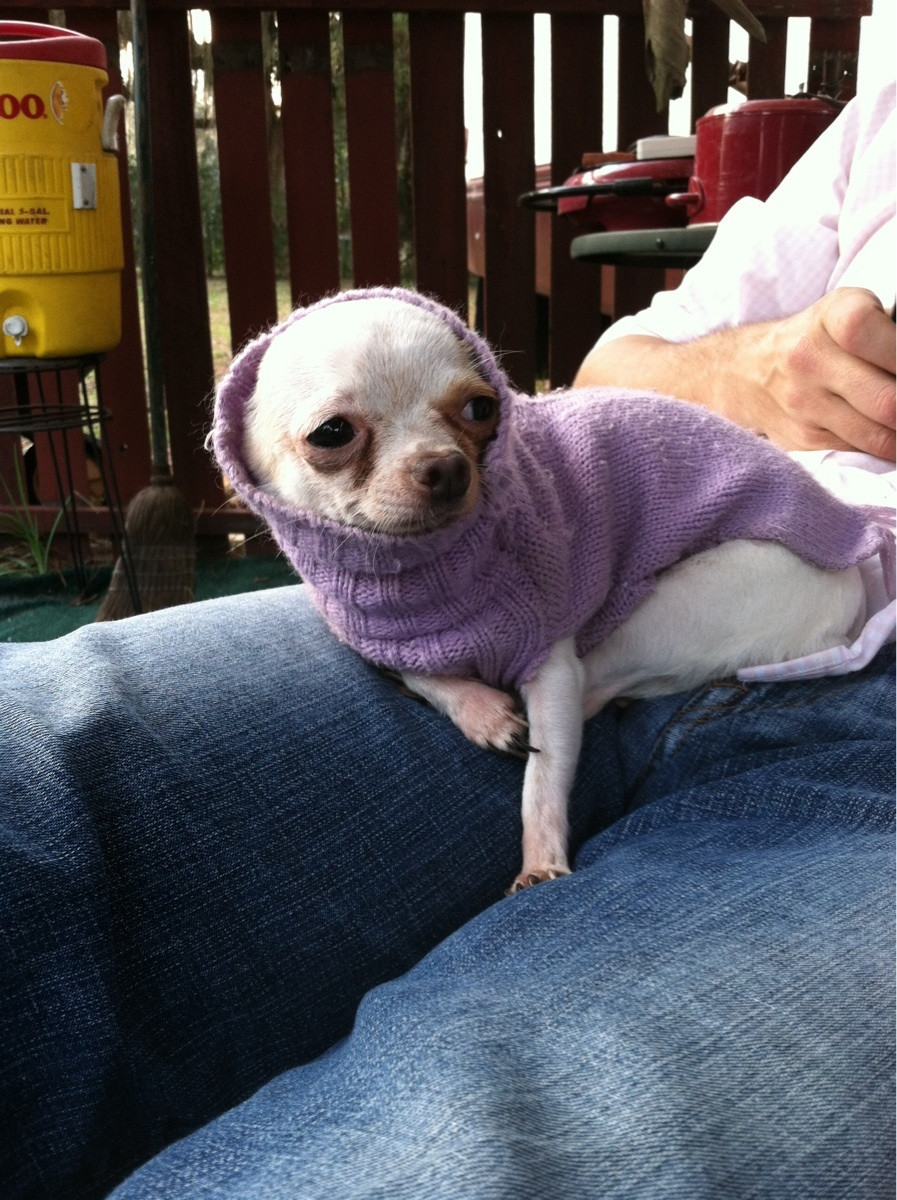
\includegraphics[width=5cm]{dog.jpeg}
      \end{center}
    \end{figure}

    \column{0.5\textwidth}
    \begin{enumerate}
    \item What's the point?
      \pause
    \item It's like a rubix cube...
      \pause
    \item Perhaps more like a poem, less like a pun...
    \end{enumerate}
  \end{columns}
\end{frame}

\begin{frame}{Da Quine}
  \begin{columns}
    \column{0.5\textwidth}
    \begin{enumerate}
    \item How do you build a quine?
    \uncover<2->{\item By thinking... \emph{hard!}}
    \end{enumerate}

    \column{0.5\textwidth}
    \begin{figure}[ht]
      \begin{center}
        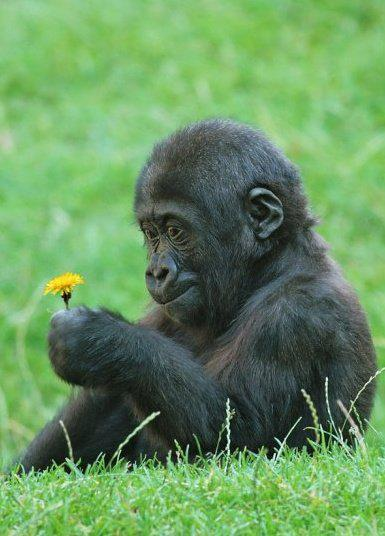
\includegraphics[height=6.5cm]{ape.jpeg}
      \end{center}
    \end{figure}    
  \end{columns}
\end{frame}

\begin{frame}[fragile]{The Quine}
\begin{verbatim}
puts ...
\end{verbatim}
\end{frame}

\begin{frame}[fragile]{The Quine}
\begin{verbatim}
puts body
\end{verbatim}
\end{frame}

\begin{frame}[fragile]{The Quine}
\begin{verbatim}
body = ...
puts body
\end{verbatim}
\end{frame}

\begin{frame}[fragile]{The Quine}
\begin{verbatim}
body = ...
puts "body = %p" % body, body
\end{verbatim}
\end{frame}

\begin{frame}[fragile]{The Quine}
\begin{verbatim}
body = "puts \"body = %p\" % body, body"
puts "body = %p" % body, body
\end{verbatim}
\end{frame}

\begin{frame}{Le Quine}
  Let's explore...
  \pause
  \begin{enumerate}
  \item Abstract
    \pause
  \item Generalize
  \end{enumerate}
\end{frame}

\begin{frame}
  Eveything would be easier if we just had a variable
  containing the source code...\pause\;say \$src
\end{frame}

\begin{frame}{The Meta-Quine}
  \begin{figure}[ht]
    \begin{center}
      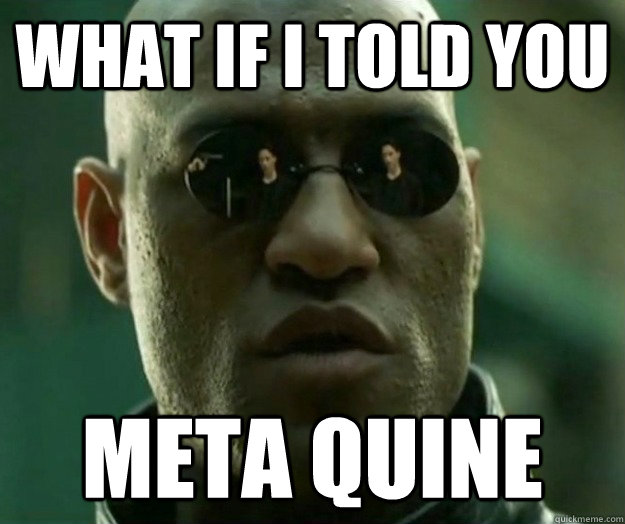
\includegraphics[height=6.5cm]{morpheus.jpeg}
    \end{center}
  \end{figure}  
\end{frame}

\begin{frame}[fragile]{The Meta-Quine for great justice}
\verbatiminput{mkquine.rb}
\end{frame}

\begin{frame}{The Meta-Quine}
  A meta quine takes a program as input and produces a new
  program which can access its own source code through the \$src
  variable.
\end{frame}

\begin{frame}{The Meta-Quine}
  With a meta-quine, we can do cool things with quines super easily...

  \pause

  In fact we can easily show that you can output any function
  of your own source code...
\end{frame}

\begin{frame}
  \begin{figure}[ht]
    \begin{center}
      
\includegraphics[height=6.5cm]{showme.jpeg}
    \end{center}
  \end{figure}  
\end{frame}

\begin{frame}{Questions}
  \begin{figure}[ht]
    \begin{center}
      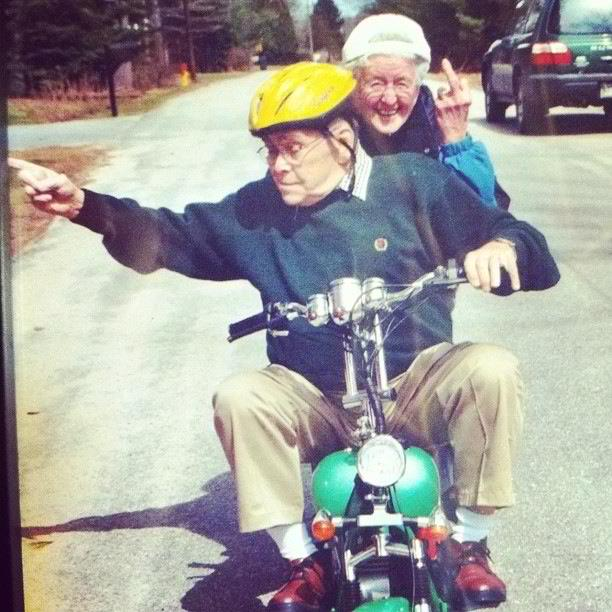
\includegraphics[height=6.5cm]{old.jpeg}
    \end{center}
  \end{figure}  
\end{frame}


\end{document}
